\documentclass[a4paper,twocolumn,11pt]{article}
\usepackage[utf8]{inputenc}
\usepackage[english]{babel}
\usepackage{graphicx}
\usepackage{biblatex}
\usepackage{cleveref}
\title{Using \LaTeX{} and Gnuplot: The Fresnel Integrals}
\author{Helene Hestbech Jørgensen}
\date{\today}
\begin{document}
\maketitle

\noindent
The Fresnel integrals are defined as the following definite integrals:
\begin{equation}\label{fres-sine}
	S(x)=\int_{0}^{x} \sin\left(t^2\right) dt,
\end{equation}
and
\begin{equation}\label{fres-cos}
	C(x)=\int_{0}^{x} \cos\left(t^2\right) dt,
\end{equation}

\noindent where $S(x)$ is called the Fresnel sine integral and $C(x)$ is called the Fresnel cosine integral. These functions are shown in the figure.

They are named after the French engineer and physicist, Augustin-Jean Fresnel (1788-1827), who originally used them in optics calculations.\

The limit of the Fresnel functions as $x$ approaches infinity are

\begin{equation}
\int_{0}^{\infty} \cos t^2 dt = \int_{0}^{\infty} \sin t^2 dt = \frac{\sqrt{2\pi}}{4} \approx 0.6267.
\end{equation}

%The maximum of $C(x)$ is about $0.977451424$. 

In some cases, the argument $t^2$ is replaced with $\pi t^2/2$ and the functions are known as normalized Fresnel integrals. These functions converge to 1/2.\\


The Fresnel integrals can be expanded in the following power series that converge for all x:
\begin{equation}
	S(x)=\sum_{n=0}^{\infty} (-1)^n \frac{x^{4n+3}}{(2n+1)!(4n+3)},
\end{equation}
and 
\begin{equation}
C(x)=\sum_{n=0}^{\infty} (-1)^n \frac{x^{4n+1}}{(2n)!(4n+1)}.
\end{equation}

The Fresnel integrals can be extended to the domain of complex numbers, $S(z)$ and $C(z)$, where they become analytic functions of a complex variable $z$ and can be expressed using the error function.

\begin{figure}[h]\label{fresnel}
% GNUPLOT: LaTeX picture with Postscript
\begingroup
  \makeatletter
  \providecommand\color[2][]{%
    \GenericError{(gnuplot) \space\space\space\@spaces}{%
      Package color not loaded in conjunction with
      terminal option `colourtext'%
    }{See the gnuplot documentation for explanation.%
    }{Either use 'blacktext' in gnuplot or load the package
      color.sty in LaTeX.}%
    \renewcommand\color[2][]{}%
  }%
  \providecommand\includegraphics[2][]{%
    \GenericError{(gnuplot) \space\space\space\@spaces}{%
      Package graphicx or graphics not loaded%
    }{See the gnuplot documentation for explanation.%
    }{The gnuplot epslatex terminal needs graphicx.sty or graphics.sty.}%
    \renewcommand\includegraphics[2][]{}%
  }%
  \providecommand\rotatebox[2]{#2}%
  \@ifundefined{ifGPcolor}{%
    \newif\ifGPcolor
    \GPcolortrue
  }{}%
  \@ifundefined{ifGPblacktext}{%
    \newif\ifGPblacktext
    \GPblacktexttrue
  }{}%
  % define a \g@addto@macro without @ in the name:
  \let\gplgaddtomacro\g@addto@macro
  % define empty templates for all commands taking text:
  \gdef\gplbacktext{}%
  \gdef\gplfronttext{}%
  \makeatother
  \ifGPblacktext
    % no textcolor at all
    \def\colorrgb#1{}%
    \def\colorgray#1{}%
  \else
    % gray or color?
    \ifGPcolor
      \def\colorrgb#1{\color[rgb]{#1}}%
      \def\colorgray#1{\color[gray]{#1}}%
      \expandafter\def\csname LTw\endcsname{\color{white}}%
      \expandafter\def\csname LTb\endcsname{\color{black}}%
      \expandafter\def\csname LTa\endcsname{\color{black}}%
      \expandafter\def\csname LT0\endcsname{\color[rgb]{1,0,0}}%
      \expandafter\def\csname LT1\endcsname{\color[rgb]{0,1,0}}%
      \expandafter\def\csname LT2\endcsname{\color[rgb]{0,0,1}}%
      \expandafter\def\csname LT3\endcsname{\color[rgb]{1,0,1}}%
      \expandafter\def\csname LT4\endcsname{\color[rgb]{0,1,1}}%
      \expandafter\def\csname LT5\endcsname{\color[rgb]{1,1,0}}%
      \expandafter\def\csname LT6\endcsname{\color[rgb]{0,0,0}}%
      \expandafter\def\csname LT7\endcsname{\color[rgb]{1,0.3,0}}%
      \expandafter\def\csname LT8\endcsname{\color[rgb]{0.5,0.5,0.5}}%
    \else
      % gray
      \def\colorrgb#1{\color{black}}%
      \def\colorgray#1{\color[gray]{#1}}%
      \expandafter\def\csname LTw\endcsname{\color{white}}%
      \expandafter\def\csname LTb\endcsname{\color{black}}%
      \expandafter\def\csname LTa\endcsname{\color{black}}%
      \expandafter\def\csname LT0\endcsname{\color{black}}%
      \expandafter\def\csname LT1\endcsname{\color{black}}%
      \expandafter\def\csname LT2\endcsname{\color{black}}%
      \expandafter\def\csname LT3\endcsname{\color{black}}%
      \expandafter\def\csname LT4\endcsname{\color{black}}%
      \expandafter\def\csname LT5\endcsname{\color{black}}%
      \expandafter\def\csname LT6\endcsname{\color{black}}%
      \expandafter\def\csname LT7\endcsname{\color{black}}%
      \expandafter\def\csname LT8\endcsname{\color{black}}%
    \fi
  \fi
    \setlength{\unitlength}{0.0500bp}%
    \ifx\gptboxheight\undefined%
      \newlength{\gptboxheight}%
      \newlength{\gptboxwidth}%
      \newsavebox{\gptboxtext}%
    \fi%
    \setlength{\fboxrule}{0.5pt}%
    \setlength{\fboxsep}{1pt}%
\begin{picture}(4500.00,3380.00)%
    \gplgaddtomacro\gplbacktext{%
      \csname LTb\endcsname%%
      \put(616,560){\makebox(0,0)[r]{\strut{}$0$}}%
      \csname LTb\endcsname%%
      \put(616,1089){\makebox(0,0)[r]{\strut{}$0.2$}}%
      \csname LTb\endcsname%%
      \put(616,1618){\makebox(0,0)[r]{\strut{}$0.4$}}%
      \csname LTb\endcsname%%
      \put(616,2146){\makebox(0,0)[r]{\strut{}$0.6$}}%
      \csname LTb\endcsname%%
      \put(616,2675){\makebox(0,0)[r]{\strut{}$0.8$}}%
      \csname LTb\endcsname%%
      \put(616,3204){\makebox(0,0)[r]{\strut{}$1$}}%
      \csname LTb\endcsname%%
      \put(714,385){\makebox(0,0){\strut{}$0$}}%
      \csname LTb\endcsname%%
      \put(1412,385){\makebox(0,0){\strut{}$1$}}%
      \csname LTb\endcsname%%
      \put(2110,385){\makebox(0,0){\strut{}$2$}}%
      \csname LTb\endcsname%%
      \put(2809,385){\makebox(0,0){\strut{}$3$}}%
      \csname LTb\endcsname%%
      \put(3507,385){\makebox(0,0){\strut{}$4$}}%
      \csname LTb\endcsname%%
      \put(4205,385){\makebox(0,0){\strut{}$5$}}%
    }%
    \gplgaddtomacro\gplfronttext{%
      \csname LTb\endcsname%%
      \put(161,1882){\rotatebox{-270}{\makebox(0,0){\strut{}$f(x)$}}}%
      \csname LTb\endcsname%%
      \put(2459,123){\makebox(0,0){\strut{}$x$}}%
      \csname LTb\endcsname%%
      \put(3449,892){\makebox(0,0)[r]{\strut{}$S(x)$}}%
      \csname LTb\endcsname%%
      \put(3449,717){\makebox(0,0)[r]{\strut{}$C(x)$}}%
    }%
    \gplbacktext
    \put(0,0){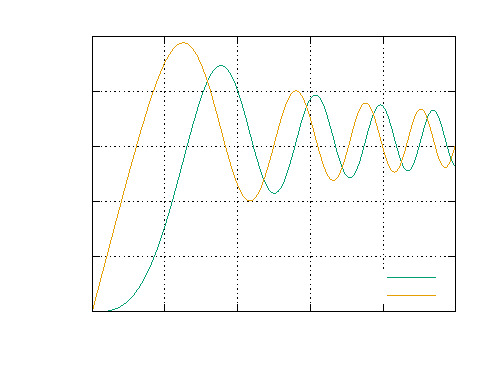
\includegraphics{Fresnel}}%
    \gplfronttext
  \end{picture}%
\endgroup

\caption{Plots of the Fresnel functions, $S(x)$ and $C(x)$.}
\end{figure}

\begin{thebibliography}{9}
	\bibitem{Wikifresnel}
	Wikipedia, Fresnel integral,
	\url{https://en.wikipedia.org/wiki/Fresnel_integral},
	accessed: 2020-05-05.
	
	\bibitem{WikiJean}
	Wikipedia, Augustin-Jean Fresnel,
	\url{https://en.wikipedia.org/wiki/Augustin-Jean_Fresnel},
	accessed: 2020-05-05.
\end{thebibliography}

\end{document}
